\onehalfspacing
\section{Đề số 27}

\begin{bt} 
   \hfill
   \begin{enumerate}[a.]
    \item Thực hiện phép tính: $A=\frac{2^{12} \cdot 3^5-4^6 \cdot 9^2}{\left(2^2 \cdot 3\right)^6+8^4 \cdot 3^5}$
    \item Cho hàm số $y=f(x)=a x^2+b x+c$.
    
    Cho biết $f(0)=2014 ; f(1)=2015 ; f(-1)=2017$. Tính $f(-2)$.
   \end{enumerate}
\loigiai{
    \begin{enumerate}
        \item $A=\frac{2^{12} \cdot 3^5-4^6 \cdot 9^2}{\left(2^2 \cdot 3\right)^6+8^4 \cdot 3^5}=\frac{2^{12} \cdot 3^5-2^{12} \cdot 3^4}{2^{12} \cdot 3^6+2^{12} \cdot 3^5} \\[5px]
        =\frac{2^{12} \cdot 3^4(3-1)}{2^{12} \cdot 3^5(3+1)}=\frac{2}{3 \cdot 4}=\frac{1}{6}$
        \item Ta có $f(0)=2014 \Leftrightarrow c=2014$
        $f(1)=2015 \Leftrightarrow a+b+c=2015 \Rightarrow a+b=1$ (1)\\[5px]
        $f(-1)=2017 \Leftrightarrow a-b+c=2017 \Rightarrow a-b=3$ (2)\\[5px]
        Từ (1)(2) suy ra: $a=2 ; b=-1$. Khi đó $f(x)=2 x^2-x+2014$\\[5px]
        Suy ra $f(-2)=2 \cdot(-2)^2-(-2)+2014=2024$
    \end{enumerate}
}
\end{bt}

\begin{bt}
   Tìm $x$, $y$ biết:
	\begin{enumerate}[a.]
        \item $\left|x+\frac{1}{5}\right|-4=-2$
        \item $2^{x-1}+5.2^{x-2}=\frac{7}{32}$
        \item $|x+5|+(3 y-4)^{2016}=0$
        \item $\frac{x}{2}=\frac{y}{5}$ và $x y=40$
    \end{enumerate}
	\loigiai{
        \begin{enumerate}
            \item $\left|x+\frac{1}{5}\right|-4=-2\\[5px] \Leftrightarrow\left|x+\frac{1}{5}\right|=2\\[5px] \Leftrightarrow\left[\begin{array}{l}x+\frac{1}{5}=2 \\[5px] x+\frac{1}{5}=-2\end{array} \Rightarrow\left[\begin{array}{l}x=\frac{9}{5} \\[5px] x=-\frac{11}{5}\end{array}\right.\right.$\\[5px]
            Vậy $x=\frac{9}{5} ; x=-\frac{11}{5}$
            \item $2^{x-1}+5 \cdot 2^{x-2}=\frac{7}{32}\\[5px] \Leftrightarrow 2^{x-1}\left(1+\frac{5}{2}\right)=\frac{7}{32} \Leftrightarrow 2^{x-1} \cdot \frac{7}{2}=\frac{7}{32} \Leftrightarrow 2^{x-1}=\frac{7}{32} \cdot \frac{2}{7}=\frac{1}{16}=2^{-4}$\\[5px]
            Suy ra $x-1=-4 \Leftrightarrow x=-3$. Vậy $x=-3$.
            \item $|x+5|+(3 y-4)^{2016}=0$. Vi $|x+5| \geq 0 ;(3 y-4)^{2016} \geq 0$\\[5px]
            Suy ra: $\left\{\begin{array}{l}|x+5|=0 \\[5px] (3 y-4)^{2016}=0\end{array} \Leftrightarrow\left\{\begin{array}{l}x+5=0 \\[5px] 3 y-4=0\end{array} \Leftrightarrow\left\{\begin{array}{l}x=-5 \\[5px] y=\frac{4}{3}\end{array}\right.\right.\right.$.\\[5px]
            Vậy $x=-5 ; y=\frac{4}{3}$
            \item Ta có: $\frac{x}{2}=\frac{y}{5}\\[5px] \Leftrightarrow \frac{x y}{2.5}=\frac{y^2}{5^2}\\[5px] \Leftrightarrow \frac{40}{10}=\frac{y^2}{25}\\[5px] \Rightarrow y^2=10^2 \Leftrightarrow y= \pm 10 \Rightarrow x= \pm 4$\\[5px]
            Vậy $(x ; y) \in\{(4 ; 10) ;(-4 ;-10)\}$
        \end{enumerate}
    } 
\end{bt}

\begin{bt}
    \hfill
    \begin{enumerate}[a.]
        \item Tìm tất cả các cặp số nguyên $x$, $y$ sao cho: $2 x y+x-2 y=4$
        \item Số $\mathrm{M}$ được chia thành ba số tỉ lệ với 0,$5 ; 1 \frac{2}{3} ; 2 \frac{1}{4}$. Tìm số $\mathrm{M}$ biết rằng tổng bình phương của ba số đó bằng 4660 .
    \end{enumerate}
	\loigiai{
        \begin{enumerate}
            \item $\text { 1) Ta có: } 2 x y+x-2 y=4 \Leftrightarrow x(2 y+1)-(2 y+1)=3 \Leftrightarrow(x-1)(2 y+1)=3 \\[5px]
            \Leftrightarrow(x-1)(2 y+1)=3=( \pm 1) \cdot( \pm 3)=( \pm 3) \cdot( \pm 1)$\\[5px] 
            $\begin{array}{|c|c|c|c|c|}
                \hline x-1 & 1 & -1 & 3 & -3 \\[5px]
                \hline x & 2 & 0 & 4 & -2 \\[5px]
                \hline 2 \mathrm{y}+1 & 3 & -3 & 1 & -1 \\[5px]
                \hline \mathrm{y} & 1 & -2 & 0 & -1 \\[5px]
                \hline
                \end{array}$\\[5px] 
            Vậy $(x ; y) \in\{(2 ; 1) ;(0 ;-2) ;(4 ; 0) ;(-2 ;-1)\}$
            \item Ta có $0,5: 1 \frac{2}{3}: 2 \frac{1}{4}=\frac{1}{2}: \frac{5}{3}: \frac{9}{4}=\frac{6}{12}: \frac{20}{12}: \frac{27}{12}=6: 20: 27$\\[5px]
            Giả sử $\mathrm{M}$ được chia thành 3 số là $x ; y ; z$.\\[5px] 
            Theo bài ra ta có:\\[5px]
            $\frac{x}{6}=\frac{y}{20}=\frac{z}{27} \Leftrightarrow \frac{x^2}{6^2}=\frac{y^2}{20^2}=\frac{z^2}{27^2}=\frac{x^2+y^2+z^2}{6^2+20^2+27^2}=\frac{4660}{1165}=4=2^2 \\[5px]           
            \Rightarrow x^2=12^2 \Rightarrow x= \pm 12 ; y^2=40^2 \Rightarrow y= \pm 40 ; z^2=54^2 \Rightarrow z= \pm 54 \\[5px]         
            \text {Vậy } M=12+40+54=106 \text { Hoặc } M=-12-40-54=-106$
        \end{enumerate}
    }
\end{bt}

\begin{bt}
    Cho tam giác $\mathrm{ABC}$ cân tại $\mathrm{A}$. Trên cạnh $\mathrm{BC}$ lấy điểm $\mathrm{D}$, trên tia đối của tia $C B$ lấy điểm $E$ sao cho $C E=B D$. Đường thẳng vuông góc với $B C$ kẻ từ $\mathrm{D}$ cắt $A B$ tại $M$. Đường vuông góc với $\mathrm{BE}$ tại $\mathrm{E}$ cắt $\mathrm{AC}$ tại $\mathrm{N}$.
    \begin{enumerate}[a.]
        \item Chứng minh: $\triangle M B D=\triangle N C E$.
        \item Cạnh $\mathrm{BC}$ cắt $\mathrm{MN}$ tại $\mathrm{I}$. Chứng minh $\mathrm{I}$ trung điểm của $\mathrm{MN}$.
        \item Chứng minh đường thẳng vuông góc với $\mathrm{MN}$ tại $\mathrm{I}$ luôn đi qua một điểm cố định khi D thay đổi trên đoạn BC.
    \end{enumerate}
	\loigiai{
        $$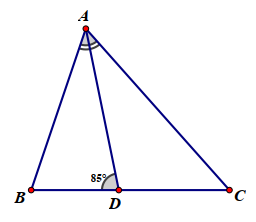
\includegraphics[width=0.4\textwidth]{13-4-lg.png}$$
        \begin{enumerate}
            \item Ta có $A B C=N C E=(A C B)$\\[5px]
            $\Rightarrow \triangle M B D=\triangle N C E(c g v-g n) \text {. }$
            \item Theo câu a)\\[5px]
            $\Rightarrow M D=E N \Rightarrow \triangle I M D=I N E(c g v-g n) \Rightarrow I M=I N \Rightarrow I \text { trung điểm } \mathrm{MN} \text {. }$\\[5px]
            \item $\text {Kẻ } A H \perp B C \\[5px]
            \Rightarrow \triangle A B H=\triangle A C H(c h-g n) \\[5px]
            \Rightarrow B A H=C A H$\\[5px]
            Đường vuông góc với $\mathrm{MN}$ tại $\mathrm{I}$ cắt $\mathrm{AH}$ tại $\mathrm{O}$.\\[5px]
            $\Rightarrow \triangle O A B=\triangle O A C(\text { c.g.c) } \\[5px]
            \Rightarrow O B A=O C A\\[5px]$
            Mặt khác :\\[5px]
            $\triangle O B H=\triangle O C H(2 c g v) \Rightarrow O B=O C (*)\\[5px] 
            \triangle O M I=\triangle O N I(2 c g v) \Rightarrow O M=O N (**)\\[5px]
            B M=C N \text { (câu b) }\left(^{* * *}\right)\\[5px]$
            Từ $\left({ }^*\right)\left({ }^{* *}\right)\left({ }^{* *}\right)$ suy ra :\\[5px]
            $\triangle O B M=\triangle O C N(\text { c.c.c }) \Rightarrow O B M=O C N$
            Từ (2)(3) $\Rightarrow O C A=O C N(=O B A)=90^{\circ} \Rightarrow O C \perp A C$\\[5px] 
            Vì $\mathrm{AC}$ cố định mà $O C \perp A C \Rightarrow \mathrm{O}$ cố định.\\[5px]
            $\text { Vậy đường thẳng vuông góc với } \mathrm{MN} \text { tại } \mathrm{I} \text { luôn đi qua điểm } \mathrm{O} \text { cố định. }$
        \end{enumerate}
    }
\end{bt}

\begin{bt}
   \hfill
   \begin{enumerate}[a.]
    \item Tìm số tự nhiên có ba chữ số. Biết rằng số đó chia hết cho 7 và tổng các chữ số đó bằng 14.
    \item Cho tam giác $\mathrm{ABC}$ có $B A C=B C A=80^{\circ}$. Ở miền trong của tam giác vẽ hai tia $\mathrm{Ax}$ và $C y$ cắt $\mathrm{BC}$ và $\mathrm{BA}$ lân lượt tại $\mathrm{D}$ và $\mathrm{E}$. Cho biết $C A D=60^{\circ} ; E C A=50^{\circ}$.
    Tính số đo góc $A D E$.
   \end{enumerate}
\loigiai{
    \begin{enumerate}
        \item Ta có:\\[5px]
        $\overline{a b c}: 7 \Leftrightarrow(100 a+10 b+c) \vdots 7 \Leftrightarrow(98 a+7 b+2 a+3 b+c) \vdots 7 \Leftrightarrow(2 a+3 b+c) \vdots 7(1)$\\[5px]
        Mặt khác theo bài ra :\\[5px]
        $a+b+c=14 \Rightarrow(a+b+c) \vdots 7 \Rightarrow(2 a+2 b+2 c) \vdots 7$\\[5px]
        Từ (1), (2) $\Rightarrow b-c \vdots 7 \Rightarrow b-c \in\{-7 ; 0 ; 7\}$\\[5px]
        +) Nếu $b-c=7$ có:\\[5px]
        $c=0 \Rightarrow b=7 \Rightarrow a=7 \\[5px]
        c=1 \Rightarrow b=8 \Rightarrow a=5$\\[5px] 
        $c=2 \Rightarrow b=9 \Rightarrow a=3$\\[5px]
        +) Nếu $b-c=0$ có:\\[5px]
        $b=c=6 \Rightarrow a=2 \\[5px]
        b=c=5 \Rightarrow a=4 \\[5px]
        b=c=4 \Rightarrow a=6 \\[5px]
        b=c=3 \Rightarrow a=8\\[5px]$
        +) Nếu $b-c=-7$ có:\\[5px]
        $c=b+7 \Rightarrow b =0 \Rightarrow c=7 \Rightarrow a=7 \\[5px]
        b=1 \Rightarrow c=8 \Rightarrow a=5 \\[5px]
        b=2 \Rightarrow c=9 \Rightarrow a=3\\[5px]$\\[5px]
        Vậy có 10 số thỏa mãn : 770; 581; 392; 266; 455; 644; 833; 707; 518; 329.
        \item 
        $$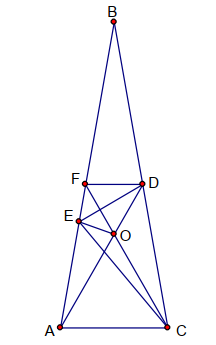
\includegraphics[width=0.35\textwidth]{27-5-lg.png}$$        
        Kẻ tia CF sao cho $A C F=60^{\circ}(F \in A B)$,
        Tia $\mathrm{CF}$ cắt $\mathrm{AD}$ tại $\mathrm{O}$.\\[5px]
        $\Rightarrow \triangle A O C ; \triangle F O D$ đều\\[5px] $\Rightarrow O A=O C=A C ; O F=O D=F D$.\\[5px]
        $\triangle A E C$ có $E A C=80^{\circ}, A C E=50^{\circ} \Rightarrow C E A=50^{\circ}$\\[5px]
        $\Rightarrow \triangle A C E$ cân tại $\mathrm{A}\\[5px] \Rightarrow A C=A E \Rightarrow \triangle A E O$ cân tại $\mathrm{A}$. Có:\\[5px]
        $E A O=20^{\circ} \Rightarrow A E O=A O E=80^{\circ} \Rightarrow E O F=40^{\circ}$\\[5px]
        Suy ra: $A F C=180^{\circ}-80^{\circ}-60^{\circ}=40^{\circ}=E O F$\\[5px]
        $\Rightarrow \triangle E O F$ cân tại $\mathrm{E} \Rightarrow E O=E F$\\[5px]
        $\Rightarrow \triangle F D E=\triangle O D E($ c.c.c)\\[5px]
        $\Rightarrow O D E=F D E=\frac{1}{2} F D A=\frac{1}{2} \cdot 60^{\circ}=30^{\circ}$ Vậy $A D E=30^{\circ}$.
    \end{enumerate}
}
\end{bt}


